\documentclass[
	english,%globale Übergabe der Hauptsprache
%	logofile=example-image-duck, %Falls die Logo Dateien nicht vorliegen
	authorontitle=true,
	]{bfhbeamer}


\usepackage[main=english]{babel}
\usepackage{caption}

% Der folgende Block ist nur bei pdfTeX auf Versionen vor April 2018 notwendig
\usepackage{iftex}
\ifPDFTeX
\usepackage[utf8]{inputenc}%kompatibilität mit TeX Versionen vor April 2018
\fi


%Makros für Formatierungen der Doku
%Im Allgemeinen nicht notwendig!
\let\code\texttt

\title{Bachelor Thesis}
\subtitle{Unlinkability of Verifiable Credentials in a practical approach}
\author[J. Robles]{Joel Robles}
\institute{TI}
\titlegraphic*{\includegraphics{example-image-duck}}%is only used with BFH-graphic and BFH-fullgraphic
\date{April 23, 2024}

% \setbeamertemplate{page number in foot}[framenumber]

%Activate the output of a frame number:
\setbeamertemplate{page number in foot}[framenumber]


\AtBeginSection{\sectionpage}

\begin{document}

\maketitle

\begin{frame}{Table of Contents}
    \tableofcontents
\end{frame}

\section{Goal}

\begin{frame}{What is the goal?}
    The goal is to analyze the BBS Signature Scheme in conjunction with VCs in concrete use-cases and to ascertain that there is no linkability or data-leakage for real-world implementations.
\end{frame}

\section{Self-sovereign Identity}

\begin{frame}{What is Self-sovereign Identity (SSI)?}
    \begin{itemize}
        \item Is a concept, where a Person, also known as a \textbf{Holder}, decides who gets to know what about them
        \item The state at the moment - Holders have no control over their data
        \item Holders cannot choose what to disclose and what not, also known as \textbf{selective disclosure}
        \item First problem: 
        \begin{itemize}
            \item Holder shows Government ID
            \item Is a set of data/ set of \textbf{attributes}
            \item The person verifying sees all the attributes
        \end{itemize}
        \item Second problem:
        \begin{itemize}
            \item Holder shows attributes to someone who wants to verify, known as a \textbf{verifier}
            \item Then shows the same attributes to a second verifier
            \item The holder then can be \textbf{linked}
        \end{itemize}
    \end{itemize}
\end{frame}

\begin{frame}{Trust Triangle}
    \begin{columns}[onlytextwidth,T]
        \column{70mm}  
        
        \begin{itemize}
            \item How does the verifier know that the set of attributes (\textbf{credential}), is valid?
            \item He trusts the issuer!
            \item Example: Swiss government ID has holograms
        \end{itemize}

        \column{70mm}

        \begin{figure}
            \centering
            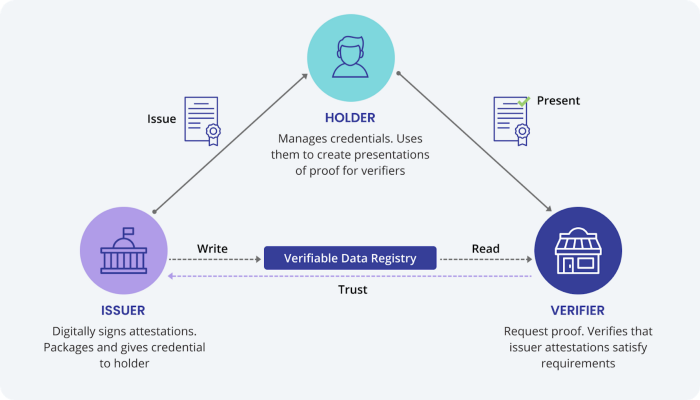
\includegraphics[width=70mm]{./img/trusttriangle.png}
            \caption{Trust triangle}
        \end{figure}
        
    \end{columns}
\end{frame}

\section{Verifiable Credentials}

\begin{frame}{Verifiable Credentials (VC)}
    \begin{columns}[onlytextwidth,T]
        \column{70mm}  

    \begin{itemize}
        \item Verifiable Credentials are digital representations of physical credentials
        \item JSON-LD represent attributes as \textbf{key-value pairs}
        \item Example:
        \begin{itemize}
            \item First name on Government ID
            \item Represented as \{"first\_name": "Joel"\}
            \item "first\_name" is the key and "Joel" is the value
        \end{itemize}
    \end{itemize}

    \column{70mm}
    \begin{figure}
        \centering
        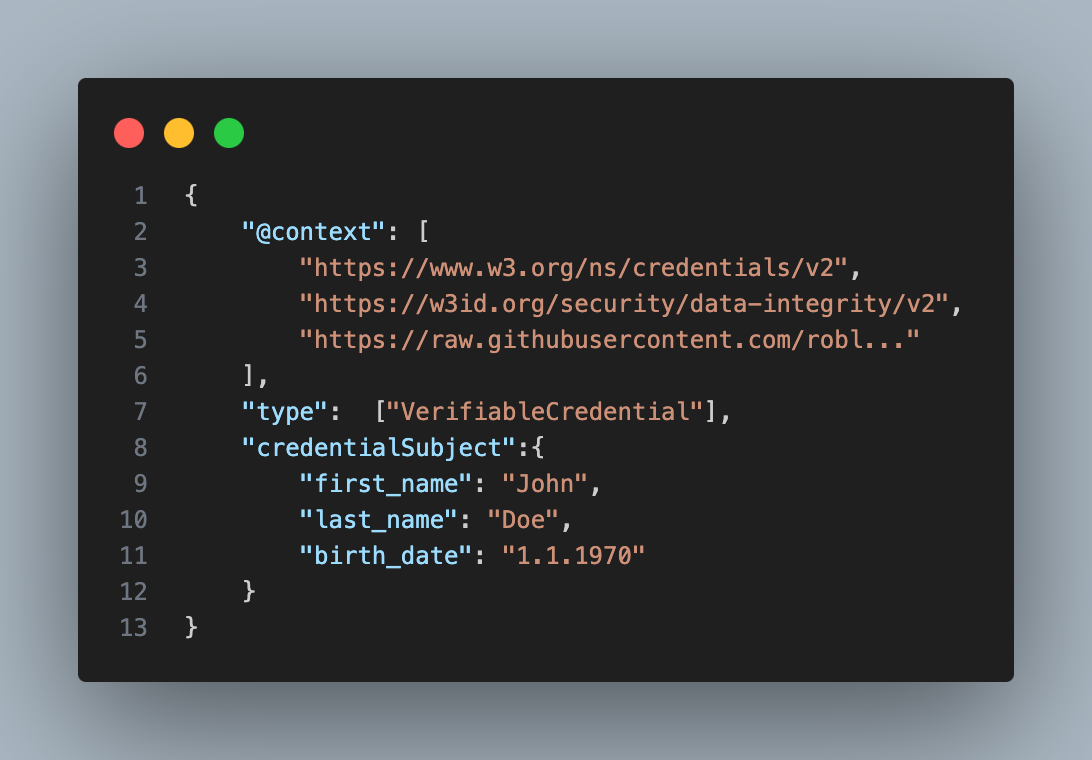
\includegraphics[width=70mm]{./img/VCexp.png}
        \caption{Example VC}
    \end{figure}

    \end{columns}
\end{frame}

\begin{frame}{VCs and BBS}
    \begin{itemize}
        \item Why are they called \textbf{Verifiable} Credentials?
        \item The verifier is able to verify a VC that was presented to him (\textbf{Verifiable Presentation}), because of cryptographic signatures
        \item These show that a credential has not been altered since issuance
        \item We use the BBS Signature Scheme (\textbf{BBS})
        \item This scheme provides \textbf{selective disclosure} and \textbf{unlinkability}
        \item How unlinkability? - Verifier needs the signature
        \item BBS can generate \textbf{proofs} 
        \item These proof that a holder knows the signature, without revealing it
        \item These are also unlinkable between each generation
    \end{itemize}
\end{frame}

\section{Verifiable Presentations}

\begin{frame}{Verifiable Presentation (VP)}
    \begin{columns}[onlytextwidth,T]
        \column{70mm}  
        \begin{itemize}
            \item A holder would like to present a VC
            \item For that, Verifiable Presentations are used
            \item BBS can only sign statements
            \item The \textbf{RDF} canonicalization algorithm creates statements out of key-value pairs
        \end{itemize}

        \column{70mm}

        \begin{figure}
            \centering
            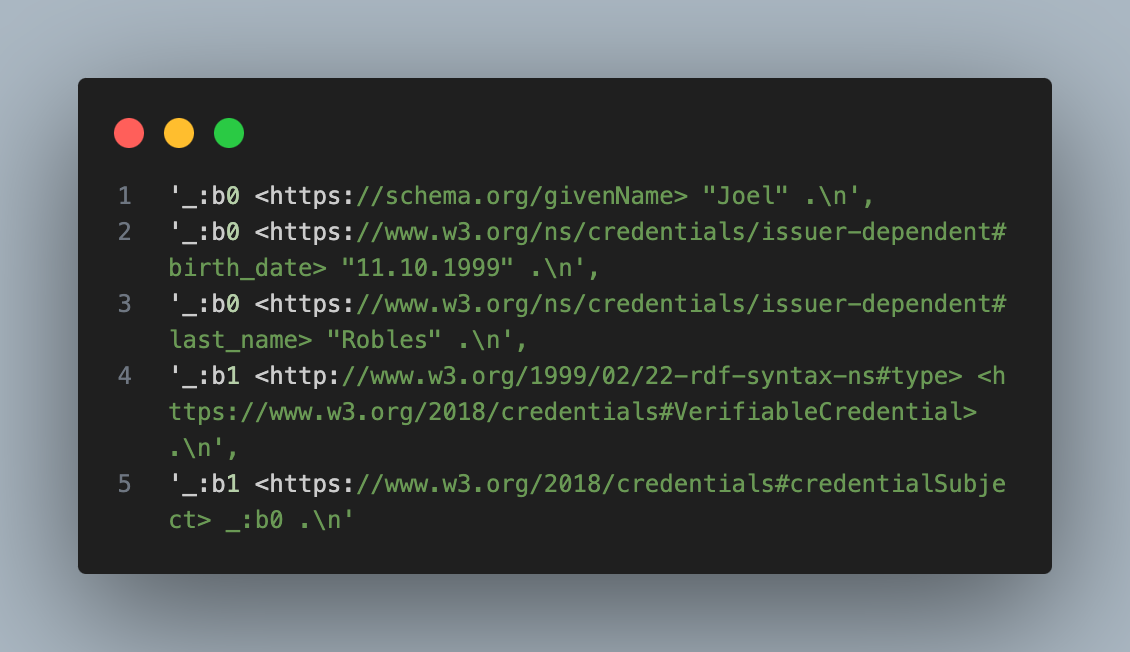
\includegraphics[width=70mm]{./img/VPcanon.png}
            \caption{Example Canonicalized VP}
        \end{figure}

    \end{columns}
\end{frame}

\section{Security Considerations}

\begin{frame}{Shuffling of statements}
    \begin{itemize}
        \item The verifier now gets a VP from the holder, which can be verified against the public key of the issuer
        \item The holder gets a new version of a credential, where an attribute has been changed
        \item In a very specific case, the RDF canonicalization algorithm can lead to data leakage
        \item Each time this algorithm is used, the canonical statements must be shuffled using a hash function
    \end{itemize}
\end{frame}

\section{Outlook}

\begin{frame}{Outlook}
    \begin{itemize}
        \item Analyze OpenID Connect for Verifiable Presentations (\textbf{OIDC4VP}) for unlinkability and data leakage
        \item Analyze Link Secrets and Blind Signatures for unlinkability and data leakage
    \end{itemize}
\end{frame}

\end{document}